\documentclass[10pt,letterpaper,twoside]{article}

\usepackage[utf8]{inputenc}
\usepackage[spanish]{babel}

\usepackage{lmodern}
\usepackage[T1]{fontenc}
\usepackage{textcomp}
\usepackage{graphicx}
\usepackage{multicol}
\usepackage{color}
\usepackage{colortbl}
\usepackage{fancyhdr}
\usepackage{hyperref}
\usepackage{float}
\usepackage{anysize}

\usepackage{epsf}
\usepackage{pdftricks}
\usepackage{pstricks}

\hypersetup{
%    bookmarks=true,
    colorlinks=true,
    linkcolor=red,
    citecolor=green,
    filecolor=magenta,
    urlcolor=blue
}

% Configuración de tamaño de página

\setlength{\parindent}{0in}
\setlength{\parskip}{0.1cm}
\setlength{\oddsidemargin}{0.05mm}
\setlength{\evensidemargin}{-20mm}

\addtolength{\textwidth}{2cm}
\addtolength{\topmargin}{-2.9cm}
\addtolength{\textheight}{4.5cm}

\pagestyle{fancy}

% Configuración de Cabeceras Fancy Header
\fancyhead{}
\fancyfoot{} % clear all footer fields
\fancyfoot[LE]{\textbf{\textsf{CIDETSI | \thepage}}}
\fancyfoot[RO]{\textbf{\textsf{\thepage | CIDETSI}}}
\renewcommand{\footrulewidth}{0.4pt}

\renewcommand{\headrulewidth}{0pt}

% Colores
\definecolor{introcolor}{rgb}{0.33,0.86,1}
\definecolor{gcolor}{rgb}{0.1,0.1,0.1}
\definecolor{listcolor}{rgb}{0.2,0.4,0.2}
\definecolor{titlecolor}{rgb}{0,0.6,0.8}
\definecolor{excolor}{rgb}{0.8,0.8,0.8}
\definecolor{notecolor}{rgb}{0.4,0.4,1.0}

\newcommand{\atext}[1]{
    \vspace{10mm}{{\textcolor{titlecolor}{\huge{\textbf{\textsf{#1}\\}}}}}
    \vspace{10mm}
}
\newcommand{\btext}[1]{
    \vspace{10mm}
    {{\textcolor{titlecolor}{\large{\textbf{\textsf{#1}}}}}}
    \vspace{5mm}
    \\
}
\newcommand{\ctext}[1]{
    \vspace{5mm}
    {{\textcolor{titlecolor}{\large{\textbf{\textsf{#1}}}}}}
    \\
}

\newcommand{\nlmsection}[4]{
{\begin{flushright}{
\colorbox{#1}{
\begin{minipage}{#3\linewidth}
\center
  \textcolor{#2}{\large{\textbf{#4}}}
\end{minipage}
}}\end{flushright}}

\vspace{4mm}
}

\newcommand{\mtitle}[2]{
  {\resizebox{#1}{0.7cm}{
    \textcolor{titlecolor}{\textbf{\textsf{#2}}}}
  }
  \vspace{1mm}
}

\newcommand{\blankpage}{
\newpage
\thispagestyle{empty}
\mbox{}
\newpage
}

\begin{document}

\pagestyle{empty}

\rput(8,-14){{\resizebox{!}{297.4mm}{\epsfbox{img/portada.eps}}}}

\clearpage
\pagebreak
\blankpage

\pagestyle{fancy}

\begin{flushright}
    \nlmsection{introcolor}{black}{0.35}{http://www.cs.umss.edu.bo}
    \mtitle{16cm}{Sitio web de las carreras de informática y sistemas}
    \\
    {\psset{linecolor=titlecolor,linestyle=dotted}\psline(-16,0)}
\end{flushright}
\vspace{5mm}

\begin{multicols}{2}
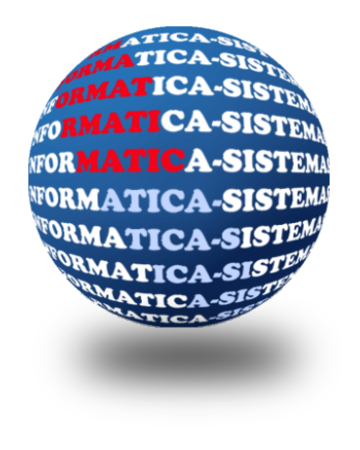
\includegraphics[scale=1.0]{img/cs.eps}

El sitio web de las carreras de informática y sistemas, fue creado con la necesidad de publicar y hacer conocer información de las carreras de informática y sistemas.

\btext{Funcionalidad del Sistema}
Las funcionalidades del sitio web de las carreras de informática y sistemas se distribuye en dos partes. La primera parte denominada parte externa accedida por todo tipo de usuario, es decir un estudiante de la carrera o una persona ajena a ella, la segunda parte denominada parte interna es la que es accedida por docentes, estudiantes, y administrador de la carrera de informática y sistemas.

\ctext{Parte Externa}
\begin{description}
\item [Reseña histórica:] Muestra al usuario datos históricos y relevantes de nuestras carreras.
\item [Biblioteca de tesis]
\begin{description}
    \item [Perfiles:] Los estudiantes y docentes deben poder observar los perfiles que aun no han defendido.
    \item [Tesis defendidas:] Es un enlace hacia el sitio web de la FCyT donde se cuenta con un banco de datos de las tesis defendidas.
    \item [Tesis libres:] Se debe manejar un historial de tesis que no llegaron a su estado final y cambio de tema.
\end{description}
\item [Plan de estudios de cada carrera:] Muestra al usuario el plan de estudios actual de cada carrera.
\item [Avisos:] Concerniente al departamento y se publicará en un lapso de tiempo que es determinado por la jefatura.
\item [Exámenes de mesa:] Que son planificados por los docentes de una materia, haciendo conocer al estudiante la fecha, hora y aula del examen, se publicará en un tiempo que es determinado por el docente.
\item [Servicios que prestamos:] Son servicios que puede ofrecer el departamento de informática y sistemas.
\begin{description}
    \item [Cursos:] posibles cursos que pueden ser organizados por el laboratorio.
    \item [Alquiler de ambientes:] los ambientes pueden ser alquilados a otras carreras o empresas.
\end{description}
\item [Eventos a realizarse:] A realizarse en el área de informática que son organizados por el departamento de informática y sistemas.
\item [Personal del departamento]
\begin{description}
\item [Docentes:] Datos de los docentes que prestan servicios a las carreras de informática y sistemas.
\item [Autoridades:] Datos de las autoridades actuales.
\end{description}
\item [Tramites:] Referente a cualquier tramite que concierna al departamento de informática y sistemas .
\item [Pasos:] Requeridos en cualquier tramite por ejemplo: tramite para el registro de perfiles.
\end{description}

\ctext{Parte Interna}
\begin{description}
\item [Aprobación de perfiles:] Pudiendo realizarse las siguientes tareas.
\begin{description}
    \item [Listado de perfiles registrados:] El docente que tenga la materia de planificación y evaluación de proyecto final podrá tener acceso a los perfiles registrados por los estudiantes.
    \item [Búsqueda:] El docente que tenga la materia de planificación y evaluación de proyecto final podrá buscar a los estudiantes que registraron sus perfiles en el sistema.
    \item [Cambios y aprobación:] El docente que tenga la materia de planificación y evaluación de proyecto final podrá aprobar los temas de perfil o habilitar para cambios los mismos.
\end{description}
\item [Avisos:] Pudiendo ser de dos tipos.
\begin{description}
    \item [Avisos del departamento:] Que son para todos los usuarios, que ingresen al sitio web de las carreras de informática y sistemas.
    \item [Avisos por materia:] Que solo serán de interés para los alumnos de una materia, pero pueden ser vistos por el público en general.
\end{description}
\item [Recursos:] Que solo serán de interés para los alumnos de una materia, pero pueden ser vistos por el público en general.
\item [Perfiles:] Pudiendo realizarse las siguientes tareas.
\begin{description}
    \item [Registro de perfiles:] El estudiante registrará su perfil en la pagina y servirá al estudiante como aval para la aprobación de su tema de tesis. El estudiante responsable podrá modificar el perfil y para dar de baja al perfil será el webmaster quien realice esta acción, la aprobación del tema lo hará el docente o el webmaster del departamento .
    \item [Aprobación de perfiles:] El docente y el webmaster tienen un listado de aquellos alumnos que tengan registrado en el sistema su perfil y podrá ver su documento final y aprobarlo.
\end{description}
\item [Correo electrónico:] Los estudiantes y docentes deben poder acceder a sus correos electrónicos por medio del sitio web de las carreras de informática y sistemas.
\item [Biblioteca:] Con la siguientes funcionalidades.
\begin{description}
    \item [Añadir temas de perfil:] Los nuevos temas de perfil deben poder ser añadidas a la biblioteca.
    \item [Añadir temas de perfil libres:] Cuando el estudiante realice un cambio de tema, su tema de perfil anterior pasara a un estado libre.
    \item [Búsquedas de perfil:] Se debe ofrecer a los estudiantes una búsqueda sobre los perfiles.
\end{description}
\item [Plan de estudios:] Con las siguientes funcionalidad.
\begin{description}
    \item [Plan de estudios de las carreras:] Se debe dar a conocer el plan de estudios actual.
    \item [Modificación del plan de estudios:] Se debe poder modificar el plan de estudios.
    \item [Enlace con los docentes:] Deben tener un enlace a una lista de docentes que dicten una materia.
\end{description}
\item [Material de una materia:] Con las siguientes funcionalidades.
\begin{description}
    \item [Subida de material de apoyo:] Un docente debe poder subir material de apoyo para su materia.
    \item [Permisos sobre el material de apoyo:] Un docente puede manejar los permisos sobre el material subido al servidor (disponible si o no).
\end{description}
\end{description}

\btext{Modulación del sistema}
Para la realización de un buen desarrollo del sistema, este se dividió en módulos los cuales mencionamos a continuación:
\begin{itemize}
    \item Módulo publico en general.
    \item Módulo administración.
    \item Módulo docente.
    \item Módulo auxiliar.
    \item Módulo estudiante.
    \item Módulo registro de perfil.
    \item Módulo autoridad.
\end{itemize}

A continuación explicaremos a mayor detalle los módulos anteriormente mencionados.

\btext{Modulo publico en general}
El modulo publico en general, tiene un propósito informativo y de comunicación entre el departamento, carreras de informática y sistemas, alumnos y publico en general que este interesado en visitar el sitio web de las carreras de informática y sistemas. Algunas de los datos que puede observar son información del departamento, de las carreras de informática y sistemas, docentes, autoridades del departamento, organigrama del departamento, tramites, tesis, perfiles, foros, plan de estudios, malla curricular de ambas carreras, materias que dicta un docente y docentes que dictan una materia y materias.

\ctext{Modulo administración}
El modulo administración se encarga de todas las operaciones que signifique una modificación a la base de datos sobre información reservada o confidencial. Algunas de las operaciones que podemos mencionar son el registro, modificación, eliminación, asignación y otros. También podemos mencionar de manera general la información que podrá modificar, como ser: departamento, carrera, tesis perfiles, servicios, avisos, información, autoridades, planes de estudio, docentes, auxiliares, estudiantes, asignación a materias, eventos, evaluación de docentes, planes globales e información del administrador.

\ctext{Modulo docente}
El modulo docente proporciona al mismo las herramientas para comunicarse con sus alumnos. Algunas de las herramientas que proporciona son: la publicación de avisos, material digital, datos del docente, evaluación de registro de perfiles, materias por carreras y la administración de notas. Debido a que la administración de notas es un subsistema, será detallada al final de este capitulo.

\ctext{Modulo auxiliar}
El modulo auxiliar proporciona al mismo la posibilidad de publicación de avisos y material digital. También podrá modificar sus datos personales.

\ctext{Modulo estudiante}
El modulo estudiante permitirá al estudiante observar los avisos y material digital que el docente les proporcione mediante el sitio web. También podrá modificar sus datos personales.

\ctext{Modulo registro de perfil}
El modulo registro de perfil permitirá al estudiante registrar su tema, modificarlo para posteriormente presentarlo en un formato requerido por el docente y por el departamento de informática y sistemas, para su aprobación final.

\ctext{Modulo Autoridad}
Podrá ver la evaluación de docentes, y la secretaria podrá publicar exámenes de mesa y normales.

\end{multicols}
\clearpage
\pagebreak
\blankpage

\begin{flushright}
    \nlmsection{introcolor}{black}{0.34}{http://sigdis.cs.umss.edu.bo}
    \mtitle{16cm}{Sistema de información para gestión de documentación de informática y sistemas}
    \\
    {\psset{linecolor=titlecolor,linestyle=dotted}\psline(-16,0)}
\end{flushright}
\vspace{5mm}

\begin{multicols}{2}

\includegraphics[scale=1.0]{img/sigdis.eps}
\newline

El sistema de información para gestión de documentación de informática y sistemas (SIGDIS) nace tras la necesidad de optimizar la gestión de documentación en el departamento de informática y sistemas. Es un sistema que tiene como objetivo principal, permitir la gestión de documentación en las carreras de ingeniería informática y de sistemas, este sistema está constituido por dos módulos, almacén y secretaria.

Es por ese motivo que SIGDIS tiene dos funciones:
\begin{itemize}
    \item Gestionar los activos asignados a los diferentes ambientes.
    \item Generar documentos emitidos en la carrera.
\end{itemize}

\btext{¿Por qué crear un nuevo sistema?}
Al comienzo y al final de cada semestre se realiza el inventariado de todos los bienes que tiene el departamento de informática y sistemas, por lo que es una tarea rutinaria y monótona en donde algunas veces se desconoce el lugar donde se encuentra ubicado algún bien o la cantidad que existe.
Es por ese motivo que se propuso crear un sistema que ayudará a realizar estas tareas, es uno de los módulos que está encargado de la gestión tanto de bienes como de ambientes, con la ayuda del sistema el usuario también puede realizar o quitar la asignación de componentes para un bien de encargados de dicha tarea, haciendo que estas tareas no consuman mucho tiempo, además con la utilización del sistema se podrá tener un seguimiento completo del bien o del componente (fecha, lugar y tiempo de utilización) el cual puede ser aprovechado en otras tareas.

La secretaria del departamento informática-sistemas cumple una función de gran importancia, debido a que es esta quien genera, maneja, y organiza la documentación correspondiente a este departamento. Es aquí donde se presenta un trabajo moroso y constante en cuanto a la generación de documentación, como ser: nombramiento de tutores, nombramiento de tribunales, nombramiento de jurados electorales, cartas de tribunales para convocatorias, cartas de adscripción, solicitudes de licencias, solicitud de corrección de resoluciones al vicerrectorado, informe de convalidaciones, certificados de egreso, entre otros; además de realizar la clasificación de esta documentación.

En secretaria es importante la clasificación de la documentación tanto recibida como enviada, con el objetivo de facilitar búsquedas posteriores para diferentes fines, de acuerdo a: fechas de emisión, tipo de documento, y otros.

Con el objetivo de facilitar el trabajo de la secretaria y mantener un respaldo digital y ordenado de la documentación es que nace la necesidad de la creación de los sistemas de gestión de documentación para la secretaria (SIGDIS).

\btext{Estructura del sistema}

\ctext{Almacén}
Es un sistema que está encargado de la gestión tanto de bienes como de ambientes, con la ayuda del sistema el usuario también puede realizar o quitar la asignación de componentes para un bien.
Con la utilización del sistema se podrá tener un seguimiento completo del bien o del componente (fecha, lugar y tiempo de utilización).
Este sistema está diseñado para facilitar el trabajo de el o los administradores de inventarios.
En resumen el sistema tiene las siguientes tareas:
\begin{itemize}
    \item Gestión de bienes.
    \item Gestión de ambientes.
    \item Asignación dinámica de componentes a un bien en particular.
    \item Filtrado de bienes por nombre o NIA.
    \item Historial de asignaciones de cada bien (indicando el lugar y tiempo al cual se encuentra asignado actualmente).
    \item Asignación dinámica de bienes a un ambiente especifico.
\end{itemize}

\ctext{Activos}
Es considerado activo todo bien material otorgado a una oficina o laboratorio.
\begin{description}
    \item [Crear activos:] Nos permite agregar un nuevo activo a la lista de activos del departamento.
    \item [Listar activos:] Esta opción muestra el listado de los activos que se posee, para esto hay dos opciones de reporte: activos vigentes y activos de baja. Podemos realizar búsquedas sobre el listado de ambientes disponibles de acuerdo a su nombre o NIA.
    \item [Historial de un activo:] esta funcionalidad nos muestra el historial del activo seleccionado, es decir una lista de los ambientes en los cuales se encontraba asignado éste activo y su estado actual.
    \item [Dar de baja/alta un activo:] Se posee también la funcionalidad de dar de baja o alta un activo.
\end{description}

\ctext{Ambientes}
Las funcionalidades que proporciona este módulo son:
\begin{description}
    \item [Crear ambientes:] Muestra el formulario de registro de ambientes.
    \item [Listar ambientes:] Muestra el listado de los ambientes disponibles en el Departamento, desde ésta vista podemos crear un nuevo ambiente, ademas de editarlos y eliminarlos.
    \item [Asignación de activos a un ambiente:] Asimismo desde ésta vista es posible también la asignación de activos a un determinado ambiente.
\end{description}

\ctext{Imágenes de activos}
Las funcionalidades que proporciona este módulo son:
\begin{description}
    \item [Subir nueva imagen:] Las imágenes subidas son para asignar en el momento de la creación de un activo.
    \item [Listar imágenes:] Muestra el listado de las imágenes disponibles en el sistema, teniendo también las opciones de ver, editar y eliminar (siempre y cuando esta imagen no esté siendo usada por algún activo).
\end{description}

\btext{Secretaria}
El objetivo de esta funcionalidad es de generar y organizar la documentación correspondiente a este
Departamento. Para esto cumple las siguientes tareas:

\ctext{Generación de documentos}
El objetivo de ésta funcionalidad es la automatización de la generación de cartas emitidas por el
Departamento, las opciones de documentos están basadas en los documentos mayormente usados por secretaría y son los siguientes:
\begin{itemize}
    \item Carta de adscripción.
    \item Certificado de egreso.
    \item Nombramiento de jurados electorales.
    \item Nombramiento de tutor.
    \item Nombramiento de tribunal de conocimiento.
    \item Nombramiento de tribunales.
    \item Solicitud de licencia.
\end{itemize}

\ctext{Búsqueda y listado de documentos}
Esta es la vista que nos muestra por defecto el enlace de generación de documentos, donde podemos realizar una búsqueda de documentos de acuerdo a: carrera, tipo de documento, destinatario y firma.

\ctext{Enviar mensaje}
Nos permite enviar un mensaje dentro del sistema y con usuarios que se encuentren registrados en el sistema.

\end{multicols}
\clearpage
\pagebreak

\begin{flushright}
    \nlmsection{introcolor}{black}{0.42}{http://comunicados.cs.umss.edu.bo}
    \mtitle{16cm}{Sistema de comunicados y avisos}
    \\
    {\psset{linecolor=titlecolor,linestyle=dotted}\psline(-16,0)}
\end{flushright}
\vspace{5mm}

\begin{multicols}{2}

\includegraphics[scale=1.0]{img/comunicados.eps}

\btext{Introducción}
Es innegable el avance de la tecnología en nuestro medio, tal vez más ahora que antes, el incremento de usuarios tuvo un crecimiento exponencial, y con ello las herramientas para facilitar y optimizar su trabajo.
En nuestro entorno social y económico, las pequeñas y medianas empresas buscan usar herramientas para su beneficio, estas herramientas sirven no solo para conectar computadoras, sino también personas, que por diferentes motivos pueden estar distanciados.
Los sistemas online presentan una opción muy interesante para usuarios que no pueden estar en un lugar, en un tiempo dado, o que se encuentran de viaje. Con este fin, es que las herramientas Web, son muy usadas en empresas.

\btext{Descripción del problema}
En una empresa o institución, se tienen varios cargos, varias áreas y secciones, las cuales trabajan en conjunto.
En este entorno es importante:
\begin{itemize}
    \item Crear ambiente de sinergia (la suma del todo es mayor a la suma de las partes).
    \item Evitar la entropía, de una o varias Secciones o Áreas.
\end{itemize}

\btext{¿Como hacer esto?}
\begin{itemize}
    \item Creando controles más efectivos.
    \item Optimizando procesos.
    \item Facilitando una adecuada comunicación entre Áreas/Secciones.
\end{itemize}

Los Avisos y Comunicados se los presenta de la siguiente forma:
\begin{itemize}
    \item Un Aviso/Comunicado se publica en un lugar visible, generalmente en una vitrina.
    \item Los comunicados son enviados a los encargados de Áreas/Secciones.
\end{itemize}

Pero existe un inconveniente: ¿Que pasa con las personas que no leen el Aviso/Comunicado en la Vitrina? . Para estos los comunicados recibidos no son difundidos.

\btext{Objetivos}

\ctext{Objetivo general}
Elaboración de un sistema de avisos y comunicados online.

\ctext{Objetivos específicos}
\begin{itemize}
    \item Desarrollo de una herramienta online, con software libre: PHP, MySQL, Apache.
    \item Recopilación de la información para el desarrollo y justificación de las herramientas, técnicas y métodos del proyecto.
\end{itemize}

\btext{Alcance}
\begin{itemize}
    \item El sistema trabaja bajo PHP-MySQL-Apache, siendo una herramienta de Internet o Intranet, debiendo estar todas estas herramientas configuradas previamente.
    \item El sistema de avisos y comunicados será una herramienta tan útil como los usuarios la aprovechen.
\end{itemize}

\btext{Justificación}
Desarrollo de herramienta de ayuda en trabajos de oficina, dando opciones a nuevas tendencias del uso de la tecnología en condiciones normales con nuevas herramientas.

\btext{¿Que se espera obtener?}
Una herramienta con la cual sea posible hacer lo siguiente:
\begin{itemize}
    \item Mandar comunicados electrónicos:
    \begin{itemize}
        \item A los docentes de las materias electivas.
        \item A los consejeros de carrera.
        \item A los docentes exclusivos.
        \item Individuales al personal.
    \end{itemize}
    \item Mandar avisos electrónicos:
    \begin{itemize}
        \item A todo el personal.
    \end{itemize}
\end{itemize}

\btext{Definiciones}
\begin{description}
    \item [Aviso:] Es un documento de comunicación masivo.
    \item [Comunicado:] Es un documento de comunicación selectivo.
    \item [Organigrama:] Un organigrama es la representación gráfica de la estructura de una empresa o institución.
\end{description}

\btext{Desarrollo del sistema}
La metodología ASD es recomendable para proyectos pequeños medianos, se eligió esta metodología por los beneficios de uso de información disponible acerca de cambios para mejorar el comportamiento del software, esta metodología tiene como primer paso la definición de la misión del proyecto.

\btext{Misión}
“Desarrollar un sistema de avisos y comunicados online para la carrera de Ingeniería de Sistemas, con el Framework de desarrollo de aplicaciones web CodeIgniter”.

\btext{Tipos de usuario}
El administrador se encarga de administrar y configurar el sistema de avisos y comunicados. Ademas, se pueden crear varios tipos de usuarios, y una jerarquía de relación.

\btext{Módulo ADMIN}
Este módulo se encarga de realizar las siguientes tareas:
\begin{itemize}
    \item Administración de avisos.
    \item Administración de comunicados.
    \item Administración de actividades.
    \item Administración de usuarios.
    \item Configuración de cuentas de acceso.
    \item Configuración de cargos.
    \item Configuración de secciones.
    \item Configuración de áreas.
    \item Manejo del organigrama jerárquico de la institución.
    \item Configuración de correo electrónico.
    \item Generación de reportes.
\end{itemize}

\ctext{Administración de avisos}
En esta componente se administran todos los avisos creados por todos los usuarios, es importante mencionar que en este componente no se crearán AVISOS, eso se lo realizará en el componente Avisos del Módulo Panel.
Las funcionalidades que realiza son:
\begin{itemize}
    \item Listar todos los avisos creados dentro del sistema.
    \item Modificar avisos creados (la modificación de avisos esta limitada, ya que la intención es modificar pequeños detalles y no así, cambiar toda la información del aviso).
    \item Eliminar avisos creados.
    \item Configurar los tipos de avisos (los tipos de avisos, sirven para poder clasificarlos).
\end{itemize}

\ctext{Administración de comunicados}
En este componente se administran todos los comunicados creados por todos los usuarios, es importante mencionar que en este componente no se crearán COMUNICADOS, eso se lo realizará en el componente Comunicados del Módulo Panel.
Las funcionalidades que realiza son:
\begin{itemize}
    \item Lista de todos los comunicados creados dentro del sistema.
    \item Modificar comunicados creados (la modificación de comunicados es limitada, ya que la intención es modificar pequeños detalles y no así, cambiar toda la información del comunicado).
    \item Eliminar comunicados creados.
    \item Configurar los tipos de comunicados (los tipos de comunicados, sirven para poder clasificarlos).
\end{itemize}

\ctext{Administración de actividades}
En esta componente se administran todas las actividades creadas por todos los usuarios, es importante mencionar que en este componente no se crearán ACTIVIDADES, eso se lo realizará en el componente Actividades del Módulo Panel.
Las funcionalidades que realiza son:
\begin{itemize}
    \item Lista de todas las actividades creadas dentro del sistema.
    \item Modificar actividades creadas.
    \item Eliminar actividades creadas.
\end{itemize}

\ctext{Administración de usuarios}
En esta componente se administran todos los usuarios creados dentro del sistema.
Las funcionalidades que realiza son:
\begin{itemize}
    \item Lista de todos los usuarios creados dentro del sistema.
    \item Modificar datos de usuarios.
    \item Eliminar usuarios.
    \item Crear nuevos usuarios: la creación de cuentas para los usuarios, se la realiza en el componente CUENTAS, en el componente USUARIOS se registran los datos básicos biográficos, como nombres, apellidos, teléfono, dirección, correo electrónico.
\end{itemize}

\ctext{Configuración de cuentas de acceso}
En esta componente se administran todas las cuentas de usuarios creados dentro del sistema.
Las funcionalidades que realiza son:
\begin{itemize}
    \item Lista de todos las cuentas creadas dentro del sistema.
    \item Modificar la información de la cuenta de acceso de los usuarios.
    \item Eliminar cuentas de usuarios.
    \item Crear nuevas cuentas de usuario.: al crear un CUENTA de usuario, se relaciona a un usuario, con un Cargo, con diferentes Secciones, Áreas. Además de poder asignarle privilegios como Admin o CRUD (creador de contenido), no todos los usuarios pueden crear Avisos/Comunicados. Ya que algunos solo podrán leer el contenido de los Avisos/Comunicados y no crearlos.
\end{itemize}

\ctext{Configuración de cargos}
En esta componente se administran todos los cargos dentro del sistema.
Puede crearse cualquier numero de cargos, pero el cargo mínimo e inicial es Admin, la creación de nuevos cargos sigue un orden jerárquico dentro de la institución.
Las funcionalidades que realiza son:
\begin{itemize}
    \item Lista de todos los cargos creados dentro del sistema.
    \item Modificar la información de los cargos.
    \item Eliminar cargos existentes u obsoletos.
    \item Crear nuevos cargos.
\end{itemize}

\ctext{Configuración de secciones}
En esta componente se administran todos las secciones dentro del sistema.
Las funcionalidades que realiza son:
\begin{itemize}
    \item Lista de todas las secciones creadas dentro del sistema.
    \item Modificar la información de las secciones.
    \item Eliminar secciones existentes u obsoletas.
    \item Crear nuevas secciones: Para la agrupación de diferentes secciones se usa el campo área, el cual se administra en el componente AREA. El campo nivel, código SIS, son exclusivas para secciones que son usadas como materias de la carrera.
\end{itemize}

\ctext{Configuración de áreas}
En esta componente se administran todas las áreas dentro del sistema.
Las funcionalidades que realiza son:
\begin{itemize}
    \item Lista de todas las áreas creadas dentro del sistema.
    \item Modificar la información de la áreas.
    \item Eliminar áreas existentes u obsoletas.
    \item Crear nuevas áreas.
\end{itemize}

\ctext{Manejo del organigrama jerárquico de la institución}
En esta componente se administra la imagen del organigrama de la carrera. La única funcionalidad que posee es permitir subir al servidor una imagen del organigrama de la carrera.

\ctext{Configuración de correo electrónico}
Se configuran los datos de correo electrónico para el envió de mensajes a los usuarios del sistema.
La única funcionalidad que posee es configurar los datos de cuenta de correo electrónico (se configuran los datos como cuenta de email, password, servidor, puerto, además los mensajes que llegaran a los usuarios).

\ctext{Generación de reportes}
Funcionalidad encargada de la generación de reportes de uso del sistema.

\btext{Módulo PANEL}
El módulo Panel es donde los usuarios podrán leer y crear AVISOS, COMUNICADOS, y ACTIVIDADES.
Este módulo se encarga de las siguientes tareas:
\begin{itemize}
    \item Administración de avisos.
    \item Administración de comunicados.
    \item Administración de actividades.
    \item Gestión de calendario.
\end{itemize}

\ctext{Administración de avisos}
En esta componente se leen y administran los avisos creados por el usuario.
Las funcionalidades que realiza son:
\begin{itemize}
    \item Lista de avisos por leer.
    \item Leer un determinado aviso.
    \item Crear aviso: Solo puede crear avisos el usuario que tenga habilitado ese privilegio.
    \item Modificar aviso: Solo el creador del aviso puede modificar la información contenida en este.
    \item Eliminar avisos. Solo el creador puede eliminar el aviso.
\end{itemize}

\ctext{Administración de comunicados}
En esta componente se leen y administran los comunicados creados por el usuario.
Las funcionalidades que realiza son:
\begin{itemize}
    \item Lista de comunicados por leer.
    \item Leer un determinado comunicado.
    \item Crear comunicado: Solo puede crear comunicados el usuario que tenga habilitado ese privilegio.
    \item Modificar comunicados: Solo el creador del comunicado puede modificar la información contenida en este.
    \item Eliminar comunicados: Solo el creador puede eliminar el comunicado.
\end{itemize}

\ctext{Administración de actividades}
En esta componente se registran actividades, creadas por usuarios.
Las funcionalidades que realiza son:
\begin{itemize}
    \item Crear una actividad.
    \item Modificar actividad es: Solo el creador de la actividad puede modificar la información contenido en esta.
    \item Eliminar actividad es: Solo el creador puede eliminar la actividad.
\end{itemize}

\ctext{Gestión de calendario}
En esta componente se visualizan las actividades registradas.
La única funcionalidad que posee es posibilitar ver el calendario con las actividades registradas.

\btext{Módulo ORGANIGRAMA}
Información sobre el organigrama, cargos, y secciones de la carrera.
Este módulo se encarga de las siguientes tareas:
\begin{description}
    \item [Organigrama de sección:] Muestra a los usuarios en las diferentes secciones que trabajan.
    \item [Organigrama de cargo:] Muestra a los usuarios en sus diferentes cargos.
    \item [Organigrama de general:] Muestra una imagen del organigrama de la carrera, esta imagen es cargada desde la componente Admin.
\end{description}

\end{multicols}
\clearpage
\pagebreak

\begin{flushright}
    \nlmsection{introcolor}{black}{0.35}{http://sapti.cs.umss.edu.bo}
    \mtitle{16cm}{Sistema de apoyo al proceso de titulación}
    \\
    {\psset{linecolor=titlecolor,linestyle=dotted}\psline(-16,0)}
\end{flushright}
\vspace{5mm}

\begin{multicols}{2}

\includegraphics[scale=1.0]{img/sapti.eps}

\btext{Antecedentes}
El sistema “SAPTI” permitirá la eficiencia administrativa del Departamento de Informática y Sistemas en el proceso de titulación, dicho sistema servirá para gestionar el seguimiento de las asignaturas de perfil y proyecto final, registrar el seguimiento de las asignaturas, historial de revisiones y estadísticas académicas.
Existen demoras en el proceso de titulación que impiden la culminación de dicho proceso. Reflejándose en que existen muchos egresados sin título.
El Departamento de Informática y Sistemas vio la necesidad de desarrollar una aplicación la cual permita automatizar de alguna manera este proceso, tanto como la información de cada proyecto, seguimiento de la revisiones, cambios realizados, información sobre los tutores, asignación de tribunales y fechas de defensa de proyectos. De esta manera los estudiantes contarán con un apoyo que les permita obtener información acerca del estado actual del proyecto, los docentes podrán revisar el historial de la evolución del proyecto y las autoridades podrán obtener estadísticas académicas acerca del proceso de titulación.

\btext{Descripción del problema}
En la carrera de Licenciatura en Ingeniería de Sistemas existen demoras en el proceso de titulación que impiden la culminación de perfil y proyecto final del mismo. Reflejándose en la existencia de muchos egresados sin título.

\btext{Objetivos}

\ctext{Objetivo General}
Realizar un sistema de software que ayude en el proceso de titulación en la carrera de Licenciatura en ingeniería de sistemas.

\ctext{Objetivos Específicos}
El sistema será capaz de:
\begin{itemize}
    \item Documentar las actividades del proyecto SAPTI.
    \item Generar Help Desk para el sistema SAPTI.
    \item Controlar la calidad de software mediante pruebas de funcionalidad al mismo.
\end{itemize}

\btext{Justificación}
\begin{description}
    \item [Técnica:] La carrera de licenciatura en ingeniería de sistemas vio la necesidad de desarrollar un aplicación en el entorno de desarrollo de software libre, la cual permita automatizar de alguna manera todo este proceso tanto como la información de cada proyecto, el seguimiento, las evaluaciones, y cambios realizados, información sobre los tutores, asignación de tribunales y fechas de defensa de proyectos.
    \item [Económica:] La aplicación será desarrollada en un entorno de desarrollo de software libre la cual representará un costo mínimo de recursos para la institución y los usuarios beneficiados.
    \item [Social:] Para facilitar el proceso de titulación de los estudiantes de la carrera de licenciatura en ingeniería de sistemas. Se espera que al desarrollar este sistema, se pueda ofrecer mayor organización entre las partes involucradas al realizar el proceso de titulación tanto en la elaboración del perfil como en el proyecto final y la defensa del mismo así garantizar la titulación al estudiante.
\end{description}

\btext{Alcances}
El sistema a desarrollar permitirá agilizar el proceso de titulación para la carrera licenciatura en ingeniería de sistemas de la universidad mayor de san simón en los siguientes casos:
\begin{itemize}
    \item El sistema manejará distintos tipos de usuarios según sus roles en el proyecto, siendo estos administrativos, tutores, tribunales, docentes y estudiantes.
    \item Seguimiento a perfiles registrados.
    \item El sistema ofrecerá una plataforma de trabajo para la coordinación de modificaciones y cambios en los proyectos.
    \item Información de proyectos en proceso.
    \item El sistema controlará las fechas de los proyectos según las normas establecidas para el proceso de titulación.
    \item El sistema será capaz de ofrecer reportes de cambio de temas, proyectos terminados, proyectos en proceso y proyectos abandonados.
    \item El sistema será capaz de asignar y sugerir nuevos tribunales adecuados según el área del proyecto elegido, sin sobrecargar a los mismos.
    \item El sistema se regirá a la normativa de la gestión I y II/2013.
\end{itemize}

\btext{Requerimientos}
Se han definido los siguientes requerimientos:

\begin{description}
    \item [Registro de evaluaciones de docentes:] Diseño e implementación del registro de evaluaciones y revisiones de cada proyecto por el docente de la materia de proyecto final.
    \item [Registro de observaciones:] Diseño e implementación del registro de revisiones de cada proyecto por el docente de la materia de proyecto final.
    \item [Listado de observaciones:] Realizadas por el docente de proyecto final a los proyectos realizados.
    \item [Modificación de observaciones:] Diseño e implementación de interfaces de usuario para la modificación de observaciones realizadas.
    \item [Registro de estudiantes:] El administrador del sistema registra a un usuario del tipo estudiante en el sistema.
    \item [Asignación de estudiantes:] El administrador asigna estudiantes a la materia "Proyecto Final".
    \item [Importación del registro de estudiantes:] El docente de la materia "Proyecto Final" importa un archivo de texto que contiene los datos de estudiantes, y el sistema asigna esos estudiantes a su materia.
    \item [Modificación de información del proyecto:] El estudiante registra cambios o correcciones de su proyecto.
    \item [Asignación de tribunales:] El consejo llena los datos de formulario para el registro de los tribunales del proyecto seleccionando introduciendo a la base de datos.
    \item [Modificación de registros de tribunales:] Permite realizar la modificación de los registros de tribunales.
    \item [Eliminación de registros de tribunales:] El sistema le permitirá la eliminación de los registros de la asignación de los tribunales.
    \item [Seguimiento de proyectos:] Mostrar en una lista los proyectos con sus respectivos tribunales y el actual estado de cada proyecto.
    \item [Buscador de los proyectos:] Permite obtener el proyecto buscado para ver el estado actual.
    \item [Registro de evaluaciones:] Permite el registro de los observaciones de cada proyecto en los respectivos tribunales.
    \item [Registro de autoridades:] Le permite el registro de las autoridades de la carrera y escribir a la base de datos.
    \item [Modificación del registro de autoridades:] Permite modificar los registros de los autoridades.
    \item [Eliminación de registro de autoridades:] Permite eliminar registros de las autoridades de la carrera de Ingeniería de sistemas.
    \item [Asignación de permisos:] Realiza la asignación de los permisos por tipos de usuarios, dando acceso a los diferentes módulos del sistema.
    \item [Modificación de registros de usuarios:] Permite realizar la modificación o cambios realizados por cada usuario. Los usuarios modifican los campos con nuevos datos.
    \item [Eliminación de registros de usuarios:] Permite realizar la eliminación de los registros de cualquier usuario ya sea docente, tutor o estudiante.
    \item [Control del proyecto:] Permite el control de los perfiles que están siendo realizados por los estudiantes o que está paralizados. Los perfiles deben estar debidamente registrados en el sistema.
    \item [Visualización de perfiles:] Permite visualizar los perfiles en una lista. Los perfiles deben estar debidamente registrados en el sistema .
    \item [Habilitación de perfil:] Permite ver los perfiles aprobados para su siguiente etapa. Los perfiles aprobados o que no tengan ninguna observación serán habilitados al siguiente proceso final.
    \item [Busqueda de tutores:] Permite mostrar en una lista los tutores disponibles. Cada perfil debe estar registrado con el área correspondiente a la que pertenece.
    \item [Asignación de tutores:] Permite la asignación según la afinidad del área y el cargo de trabajo. La asignación debe ser equitativa y organizada.
    \item [Selección de archivos en formato pdf:] Función que permite subir los archivos ya sea pdf del proyecto o sus avances. Los archivos deberán estar organizados.
    \item [Subida de archivos o documentos:] Una vez subido el archivo el sistema muestra en una lista los archivos. La subida de archivos puede ser realizada por cualquier usuario.
    \item [Mostrar documentos o perfiles:] Una vez subido el archivo el sistema muestra una lista de los archivos. Las listas deben ser organizadas.
    \item [Búsqueda de perfiles registrados:] El sistema permitirá la búsqueda de perfiles registrados ya sea esta de forma básica o avanzada. Las búsquedas se la realizan por palabras claves.
    \item [Control de duplicidades de perfil:] Muestra si existe perfiles con el mismo tema. No se permiten perfiles con el mismo tema.
    \item [Registro del perfil:] El encargado de registro perfil seleccionará la opción del menú “registro perfil”, verá el formulario para poder registrar un perfil.
    \item [Modificación de registros de perfil:] El encargado de registro perfil podrá modificar los datos ingresados al formulario para poder registrar el perfil. Implementación llenado perfil por parte del estudiante: El estudiante implementa el llenado de registro perfil en digital de dicha página.
    \item [Control de perfiles revisados:] El encargado de registro perfil podrá ver los perfiles revisados por el docente y tutores.
    \item [Aprobación de perfil por docente y tutor:] El encargado de registro perfil podrá dar visto bueno de aprobación para poder habilitar al proyecto final.
\end{description}

\btext{Funciones administrativas}
\begin{itemize}
    \item Como administradores podemos crear usuarios ver listas de todos los usuarios, modificar, configuraciones del sistema como también darles permisos, ver reportes estadísticas.
    \item En configuraciones para el sistema SAPTI se pueden registrar materias, semestres, grupo, docentes y estudiantes.
    \item Se debe crear un área y subárea para poder luego registrarse el estudiante.
    \item El administrador puede asignar a un grupo o sacarle del grupo para estar en la lista de ese grupo que se le asigna grupos a usuarios.
    \item Luego de registrar a un docente se le debe asignar en el semestre: una materia a un docente y en un grupo para que el estudiante se pueda inscribir seleccionando al grupo y a la materia que se inscribirá.
    \item Al momento de registrar estudiante se debe seleccionar en el semestre, la materia que esta inscrito, el grupo en que esta inscrito y seleccionar el titulo que tenga el estudiante.
    \item Para que un usuario pueda tener ingreso con sus cuentas los usuarios el administrador debe dar permiso necesarios. Se ingresa a permisos para ingresar a la gestión de permisos, buscar, y darle los permisos que se necesite para los usuarios que utilicen el sistema.
    \item Al ingresar a uno de los grupos en la columna PERMISOS nos mostrara la pagina de asignación de permisos en la columna tiene acceso al modulo que quiera darse acceso.
    \item El administrador debe asignar tutor que el estudiante solicito y fue aceptado ser tutor.
    \item Una vez que el estudiante solicito un tutor y fue aceptado la solicitud el administrador asignara tutor al estudiante.
\end{itemize}

\btext{Funciones según el tipo de usuario}

\ctext{Consejo de carrera:}
\begin{itemize}
    \item Los que pertenecen al honorable consejo de carrera puede ingresar con la cuenta creada por el administrador y también puede modificar su cuenta.
    \item Una vez dentro del menú consejo se puede hacer la asignación de tribunales, en el formulario de registro de tribunales se busca al estudiante por su código SIS, una vez encontrado se puede asignar automáticamente por el área en el que apoya al proyecto y su tiempo, y luego se le envía un mensaje de que fueron asignados como tribunal de los estudiantes.
\end{itemize}

\ctext{Docente:}
\begin{itemize}
    \item Se registra la disponibilidad de tiempo que tenga el docente para seleccionarlo como tribunal. Aquí el docente selecciona a que áreas puede apoyar como tribunal. El entorno de trabajo del docente muestra el menú de materias asignadas. Dentro de proyecto final ingresar a gestión de estudiantes para ver el seguimiento revisar y evaluar el proyecto.
    \item Ingresar a revisar nos muestra todo el contenido que le enviaron y ver su detalle de Avance.
    \item Se debe llenar la observación que se vio luego de ver revisar su contenido de avance del estudiante.
    \item El docente puede editar la observación que hizo borrando y creando otra observación.
    \item Se puede ver que el docente siendo tribunal puede también revisar su proyecto final.
\end{itemize}

\ctext{Estudiante:}
\begin{itemize}
    \item Al ingresar el estudiante con su cuenta puede ver el entorno de trabajo del estudiante.
    \item El estudiante puede rellenar su registro de formulario.
    \item Para el envió de avances al docente se debe ingresar a registro de avance, una vez dentro del registro de avance se puede ver que se pueden añadir archivos y luego subir los archivos que necesite enviar y llenar la descripción de avance.
    \item Dentro de proyecto final se tiene los archivos de correcciones se puede ver los detalles del docente que le reviso el avance de su proyecto.
    \item Una vez dentro de ver detalle se ve que se ingreso al detalle de correcciones del que reviso y se puede resolver en la observación que le dio el revisor al estudiante. Como se puede ver muestra el registro de correcciones que esta la observación que le dio el revisor al estudiante y puede volver a añadir y subir sus archivos modificados.
    \item Dentro de proyecto final se debe ingresar en los archivos de avances para ver todos sus archivos de avances. Se puede ver el detalle de avance que hizo el estudiante.
    \item Dentro de proyecto final se debe ingresar en los archivos de correcciones para ver todos sus archivos de correcciones.
\end{itemize}

\ctext{Tutor:}
\begin{itemize}
    \item El tutor puede ver la lista de estudiantes que enviaron solicitud de ser tutor de su proyecto del estudiante.
\end{itemize}
\end{multicols}
\clearpage

\end{document}